% chapter/Chapter.tex
\documentclass[11pt]{article}
\usepackage[margin=1in]{geometry}
\usepackage{amsmath,amssymb,graphicx,booktabs,siunitx}
\usepackage[numbers,sort&compress]{natbib}
\usepackage[hidelinks]{hyperref}
\graphicspath{{figures/}}
\title{Mathematical Models in Biotechnology}
\author{Jeffrey D. Varner\\
  Robert Frederick Smith School of Chemical and Biomolecular Engineering,\\
  Cornell University, Ithaca, NY, USA}
\date{}
\begin{document}
\maketitle
\begin{abstract}
Placeholder abstract.
\end{abstract}
%% introduction.tex
\section{Introduction}\label{sec:intro}

Biotechnology depends on predicting and directing cellular metabolism.
Metabolic engineering redirects flux toward a product. Bioprocess
development selects operating conditions that sustain production. Strain
design identifies genetic changes that alter the phenotype. Each task
requires an estimate of metabolic reaction rates under a specified condition
\cite{Bordbar2014}. These rates are difficult to measure directly. Genome
sequences and reaction annotations provide a network structure, but
reconstructions remain uncertain in reaction membership, directionality,
compartments, cofactors, and biomass composition. Fluxes, kinetic parameters,
and metabolite concentrations are even less complete at genome scale. Models
must therefore estimate phenotype from incomplete measurements. Bioprocess
models use several levels of biological detail. Unstructured
models track biomass, extracellular substrates, and products with lumped
growth, uptake, and production rates. Monod growth, inhibition, maintenance,
and growth-associated production laws support batch, fed-batch, and
continuous reactor analysis, but do not resolve intracellular fluxes
\cite{Esener1983}. Structured kinetic models add intracellular pools,
enzymes, or cellular machinery. Early single-cell models from Shuler and
coworkers coupled intracellular metabolism to extracellular nutrients in
microbial and mammalian cells \cite{Domach1984,Wu1992}. Reaction-level
kinetic models assign mass-action, Michaelis--Menten, or power-law rates to
individual reactions and integrate the resulting differential equations
\cite{MichaelisMenten1913,Savageau1976,SavageauVoit1987,Vadhin2026}. These
models describe transient intracellular behavior, but require more kinetic
parameters as their resolution increases.

Constraint-based models use a different closure. They impose mass
conservation on the reaction network and require fewer explicit kinetic
parameters. This approach can be applied to genome-scale reconstructions
\cite{Bordbar2014,AllenPalsson2003}. Flux balance analysis (FBA) formulates
the calculation as a linear program \cite{Orth2010,Heirendt2019}.
Conservation alone usually permits many flux distributions. Reaction bounds
restrict this feasible set, and an objective selects an optimum. Bounds are
a major route by which condition-specific thermodynamic, kinetic,
expression, and regulatory data enter the model. This chapter examines how
each type of data changes a bound and its predicted fluxes. The chapter first
derives the flux constraint from a mole balance, including
the growth-dilution balance $\mathbf S\hat{\mathbf v}=\mu\mathbf x$, where
$\mathbf S$ is the stoichiometric matrix, $\hat{\mathbf v}$ is the
intracellular flux vector, $\mu$ is the growth rate, and $\mathbf x$ is the
intracellular concentration vector. It then
factors each reaction bound into terms for reversibility, enzyme capacity,
substrate saturation, enzyme abundance, and regulation. Two small examples
show how these terms affect a flux prediction. The first uses public data to
set bounds in a urea-cycle network. The second transfers expression and
metabolite states from a kinetic feedback model into an FBA bound. Two larger
studies illustrate related methods in dynamic cell-free protein synthesis
\cite{Dai2018,Vilkhovoy2023} and model-guided strain design \cite{Wayman2019}.
Strain design also requires a discrete search over candidate interventions,
often formulated as a bilevel optimization problem \cite{Burgard2003}.

\section{Kinetic and Mechanistic Models}\label{sec:kinetics}
Placeholder.

\section{Flux Balance Analysis}\label{sec:fba}

Kinetic models of the type developed in Section~\ref{sec:kinetics} require
mechanistic rate expressions and numerical values for every kinetic parameter.
For large metabolic networks -- modern genome-scale reconstructions contain
thousands of reactions and metabolites \cite{Thiele2013} -- this level of
mechanistic detail is rarely available.  Flux balance analysis (FBA) circumvents
this limitation by replacing differential equations with an algebraic
constraint: at metabolic steady state the net rate of production of every
intracellular metabolite is zero.  Given only the network stoichiometry and
bounds on individual reaction rates, the optimal flux distribution consistent
with that constraint can be found by linear programming \cite{Orth2010}.

%-----------------------------------------------------------------------
\subsection{Metabolism as a Constraint-Based Problem}
%-----------------------------------------------------------------------

The stoichiometry of a metabolic network is encoded in the
\emph{stoichiometric matrix} $\mathbf{S} \in \mathbb{R}^{m \times r}$, where $m$
is the number of metabolites and $r$ is the number of reactions.  The entry
$S_{ij}$ is the stoichiometric coefficient of metabolite $i$ in reaction $j$:
negative if metabolite $i$ is consumed, positive if it is produced, and zero
otherwise.  The vector $\mathbf{v} \in \mathbb{R}^{r}$ collects the fluxes of
all reactions, in units of, for example, mmol per gram dry weight per hour.

Writing mole balances for each intracellular metabolite in a well-mixed
compartment of volume $V$ gives the dynamic equation
\begin{equation}\label{eq:fba_dynamic}
  \frac{d\mathbf{x}}{dt} = \mathbf{S}\,\mathbf{v} - \mu\,\mathbf{x},
\end{equation}
where $\mathbf{x}$ is the vector of intracellular metabolite amounts
(concentrations in the constant-volume case) and $\mu$ is the specific growth
rate (dilution by cell growth).  Metabolic fluxes
operate on the time scale of seconds to minutes, whereas the cell-growth time
scale is hours.  On the metabolic time scale the dilution term $\mu\,\mathbf{x}$
is negligible relative to $\mathbf{S}\,\mathbf{v}$, and metabolite
concentrations reach a pseudo-steady state.  Setting
$d\mathbf{x}/dt \approx \mathbf{0}$ yields the steady-state mass-balance
constraint
\begin{equation}\label{eq:Sv0}
  \mathbf{S}\,\mathbf{v} = \mathbf{0}.
\end{equation}
The formal derivation of this constraint from open-species mole balances
is given in Appendix~\ref{sec:fba_derivation}.

Equation~\eqref{eq:Sv0} defines a \emph{null space} of feasible flux
distributions.  For any realistic network with $r > m$ the system is
underdetermined; the stoichiometric constraint alone leaves many degrees of
freedom.  Constraint-based modeling resolves this indeterminacy by (i) imposing
thermodynamic and capacity bounds on individual fluxes and (ii) selecting
among the feasible solutions via an objective function that reflects cellular
physiology \cite{Bordbar2014}.

%-----------------------------------------------------------------------
\subsection{The FBA Linear Program}
%-----------------------------------------------------------------------

Given the steady-state constraint and box bounds on each flux,
\begin{equation}\label{eq:fba_lp}
  \begin{aligned}
    \text{maximize}   \quad & \mathbf{c}^{\!\top}\mathbf{v} \\
    \text{subject to} \quad & \mathbf{S}\,\mathbf{v} = \mathbf{0} \\
                            & \mathbf{lb} \leq \mathbf{v} \leq \mathbf{ub},
  \end{aligned}
\end{equation}
where $\mathbf{c} \in \mathbb{R}^{r}$ is the objective coefficient vector.
This is a linear program, solvable in polynomial time for networks of arbitrary
size \cite{Orth2010,Heirendt2019}.

The lower and upper bounds $\mathbf{lb}$ and $\mathbf{ub}$ encode two types
of constraint.  Thermodynamic reversibility determines the sign of the lower
bound: an irreversible reaction has $lb_{j} = 0$, whereas a reversible
reaction has $lb_{j} < 0$.  Enzyme capacity imposes an upper bound through
the maximum velocity $V_{\max,j} = k_{\text{cat},j}\,[E]_{j}$, where
$[E]_{j}$ is the total enzyme concentration and $k_{\text{cat},j}$ is the
turnover number \cite{Milo2010}.

\paragraph{Exchange and transport reactions.}
A metabolic network must be coupled to its environment through
\emph{exchange reactions} (sometimes called boundary reactions), which represent
the import or export of metabolites across the system boundary.  By convention,
an exchange reaction for metabolite $i$ is written as $\emptyset \to M_i$ so
that positive flux denotes import and negative flux denotes export.  These
pseudo-reactions carry no stoichiometric coefficients for other species and
appear as isolated non-zero entries in $\mathbf{S}$.  Bounds on exchange
reactions encode the composition of the medium: setting $lb_{j} = 0$ prevents
uptake of a nutrient that is absent, while $ub_{j} = 0$ prevents secretion of
a regulated product.

\paragraph{The biological objective.}
The choice of $\mathbf{c}$ encodes the metabolic goal.  Maximizing biomass
synthesis -- setting $c_{j} = 1$ for a lumped biomass-assembly reaction -- is
the canonical choice for growth studies and underpins much of the predictive
power of genome-scale FBA \cite{Orth2010}.  In biotechnological contexts the
objective may instead be maximization of a product export flux, reflecting the
engineering goal of yield optimization.  Regardless of the choice, the linearity
of the problem guarantees a unique optimal objective value, although multiple
flux vectors may attain it.

%-----------------------------------------------------------------------
\subsection{Flux Variability Analysis and Genome-Scale Structure}
%-----------------------------------------------------------------------

Because the optimal solution to Eq.~\eqref{eq:fba_lp} is typically not unique,
\emph{flux variability analysis} (FVA) characterizes the complete set of optimal
solutions.  For each reaction $j$, FVA solves two linear programs: it minimizes
and maximizes $v_j$ subject to the FBA constraints plus the requirement that the
objective value remain at its optimum.  The resulting intervals $[v_j^{\min},
v_j^{\max}]$ identify reactions that are uniquely determined at the optimum
(zero-width intervals), reactions that are completely free within the feasible
set (wide intervals), and the so-called \emph{blocked} reactions for which the
only feasible flux is zero \cite{Heirendt2019}.

At the network level, $\mathbf{S}$ encodes the full topology of metabolism.
Its null space $\mathcal{N}(\mathbf{S})$ -- the set of all flux vectors
satisfying $\mathbf{S}\,\mathbf{v} = \mathbf{0}$ -- has dimension
$r - \mathrm{rank}(\mathbf{S})$.  The singular-value decomposition
$\mathbf{S} = \mathbf{U}\boldsymbol{\Sigma}\mathbf{V}^{\!\top}$ reveals this
structure directly: the columns of $\mathbf{V}$ corresponding to zero singular
values span $\mathcal{N}(\mathbf{S})$, while the remaining columns of
$\mathbf{V}$ span the row space.  In genome-scale models (thousands of
reactions, hundreds of metabolites) $\mathrm{rank}(\mathbf{S}) \ll r$, so the
null space is high-dimensional and the feasible solution space is correspondingly
large, motivating the use of physiological objective functions to select
biologically meaningful flux distributions \cite{Bordbar2014,Thiele2013}.

%-----------------------------------------------------------------------
\subsection{Worked Example: The Urea Cycle}
%-----------------------------------------------------------------------

To illustrate FBA concretely, we apply it to a curated model of the urea cycle
in HL-60 cells.  The network comprises 5 enzymatic reactions and 14 exchange
reactions, coupling 18 intracellular metabolites ($m = 18$, $r = 19$, so
$\mathbf{S} \in \mathbb{R}^{18 \times 19}$).

\paragraph{Reactions.}
The four canonical urea-cycle enzymes are represented:
\begin{itemize}
  \item \textbf{v1} (argininosuccinate synthetase, EC 6.3.4.5):
    $\text{ATP} + \text{Citrulline} + \text{Aspartate} \to
     \text{AMP} + \text{Diphosphate} + \text{Argininosuccinate}$;
  \item \textbf{v2} (argininosuccinate lyase, EC 4.3.2.1):
    $\text{Argininosuccinate} \to \text{Fumarate} + \text{Arginine}$;
  \item \textbf{v3} (arginase I, EC 3.5.3.1):
    $\text{Arginine} + \text{H}_2\text{O} \to \text{Ornithine} + \text{Urea}$;
  \item \textbf{v4} (ornithine transcarbamylase, EC 2.1.3.3):
    $\text{Carbamoyl phosphate} + \text{Ornithine} \to
     \text{Orthophosphate} + \text{Citrulline}$.
\end{itemize}
A nitric oxide synthase branch is also included:
\begin{itemize}
  \item \textbf{v5} (NOS, EC 1.15.13.39):
    $2\,\text{Arginine} + 4\,\text{O}_2 + 3\,\text{NADPH} + 3\,\text{H}^+ \to
     2\,\text{NO} + 2\,\text{Citrulline} + 3\,\text{NADP}^+ + 4\,\text{H}_2\text{O}$.
\end{itemize}
Exchange reactions b1--b14 allow each metabolite to enter or leave the
system at bounded rates.

\paragraph{Flux bounds.}
Reversibility is assigned from the standard Gibbs free energy of reaction
evaluated by eQuilibrator: reactions with $\Delta G^{\circ\prime} < -10$\,kJ/mol
are treated as irreversible ($lb_j = 0$); the remainder are reversible.
Capacity upper bounds are set as $V_{\max,j} = k_{\text{cat},j}\,[E]_0$ with
$[E]_0 = 0.01$\,mmol\,gDW$^{-1}$ and turnover numbers from BRENDA.  The
rate-limiting step in this parameterization is v2 (argininosuccinate lyase),
whose $k_{\text{cat}} = 3.28$\,s$^{-1}$ gives
$V_{\max,\text{v2}} = 0.0328$\,mmol\,gDW$^{-1}$\,h$^{-1}$ --- the smallest
of the five enzymatic capacity bounds (v1: 0.100, v3: 1.9, v4: 4.1, v5: 0.100)
and therefore the unique network bottleneck.

\paragraph{Objective and sign convention.}
The biological goal is to maximize urea export.  Exchange reaction b4 is
defined with the import-positive convention ($\emptyset \to \text{Urea}$), so
urea export corresponds to \emph{negative} flux through b4.  To drive b4 as
negative as possible under a maximization objective, the objective coefficient
is set to $c_{\text{b4}} = -1$: maximizing $\mathbf{c}^{\!\top}\mathbf{v}$
then minimizes $v_{\text{b4}}$, which is equivalent to maximizing the rate of
urea export.

\paragraph{Optimal flux distribution.}
The linear program \eqref{eq:fba_lp} was solved with the HiGHS solver via
JuMP.  At the optimum the entire urea-cycle backbone (v1--v4) operates at
exactly $0.0328$\,mmol\,gDW$^{-1}$\,h$^{-1}$ -- the capacity imposed by
v2 -- and the NO synthase branch (v5) carries zero flux, consistent with
arginine being fully committed to urea production.  The corresponding exchange
fluxes shuttle carbamoyl phosphate, aspartate, and ATP into the cycle while
exporting urea, fumarate, AMP, and orthophosphate.  The optimal urea-export flux
magnitude is $0.0328$\,mmol\,gDW$^{-1}$\,h$^{-1}$, confirming that the cycle
rate is limited by argininosuccinate lyase.  The full flux distribution is shown
in Figure~\ref{fig:fba}.

\begin{figure}[htbp]
  \centering
  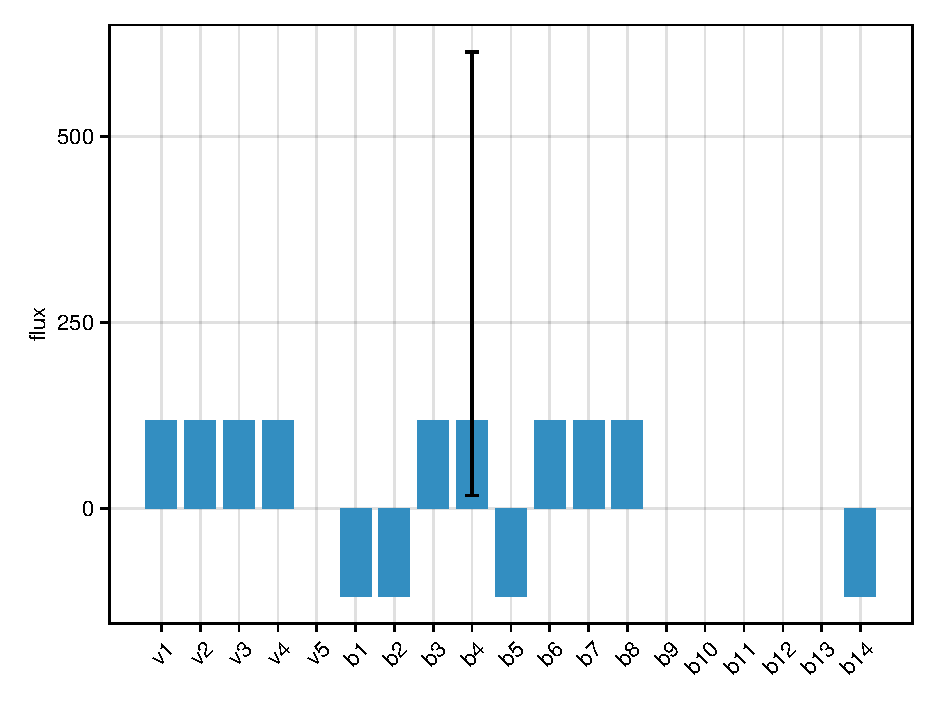
\includegraphics[width=0.85\textwidth]{urea_fba.pdf}
  \caption{Optimal flux distribution for the urea-cycle FBA model.
    Bar heights give the flux $v_j$ (mmol\,gDW$^{-1}$\,h$^{-1}$) at the
    solution of linear program~\eqref{eq:fba_lp} with the urea-export objective.
    Enzymatic reactions v1--v4 all saturate at $0.0328$\,mmol\,gDW$^{-1}$\,h$^{-1}$,
    the capacity of argininosuccinate lyase (v2).  The NO synthase branch (v5)
    carries zero flux.  Exchange reactions (b1--b14) with negative bars represent
    net export under the import-positive convention; b4 (urea) shows the
    maximized export flux of $-0.0328$\,mmol\,gDW$^{-1}$\,h$^{-1}$.}
  \label{fig:fba}
\end{figure}

\section{Models of Gene Expression}\label{sec:gene}
Placeholder.

\section{Deep Time-Series Models}\label{sec:dl}
Placeholder.

\section{Hybrid Models and Outlook}\label{sec:hybrid}
Placeholder.

\appendix
\section{Derivations}\label{sec:appendix}
Placeholder.

\bibliographystyle{unsrtnat}
\bibliography{References}
\end{document}
